\section{Risultati}\label{sec:risultati}

\subsection{Mean-field approximation}\label{subsec:res-mean-field-approximation}
    Come possiamo vedere dalla figura ~\ref{fig:mf_critical_j}, il calcolo del campo medio approssima bene il valore
    critico di $J$, sia nel caso teorico che in quello pratico, confermando la validità teorica del metodo.

    \begin{figure}[H]
        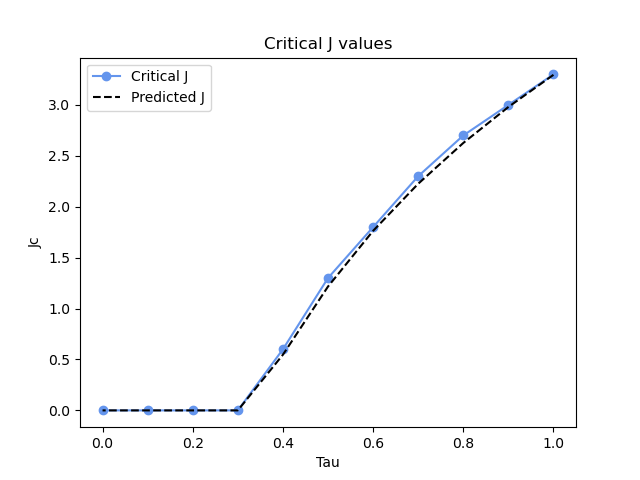
\includegraphics[width=\textwidth]{mf_critical_j}\caption{Mean-field approximation}
        \label{fig:mf_critical_j}
    \end{figure}

\subsection{Simple percolation}\label{subsec:res-simple-percolation}
    In questo caso abbiamo fatto varie simulazioni in base al numero di nodi e al valore di connettività $k$.
    I risultati mostrati in ~\ref{fig:prob_percolation} e ~\ref{fig:prob_percolation_2} mostrano i risultati ottenuti.
    Anche in questo caso siamo riusciti a ottenere che i valori predetti dalla formula sono molto vicini a
    quelli che si osservano simulando l'infezione.

    \begin{figure}[H]
        \begin{minipage}{0.5\textwidth}
            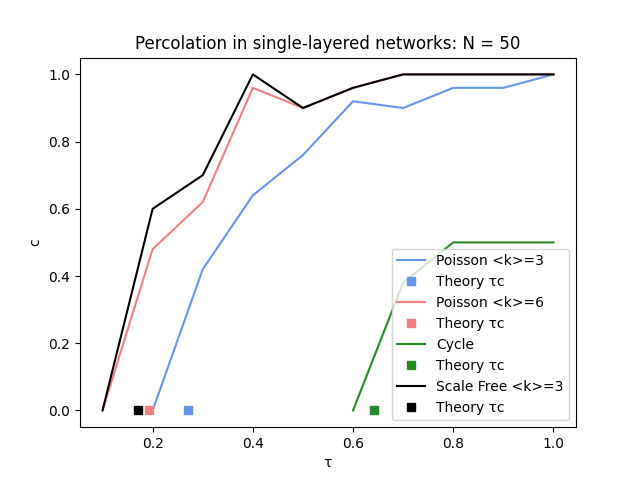
\includegraphics[width=\linewidth]{critical_t}\label{fig:prob_percolation}
        \end{minipage}
        \begin{minipage}{0.5\textwidth}
            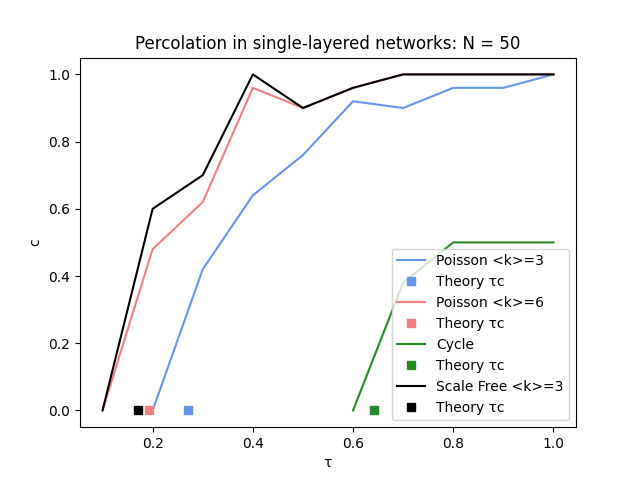
\includegraphics[width=\linewidth]{critical_t}\label{fig:prob_percolation_2}
        \end{minipage}
        \caption{Valutazione della probabilità di percolazione}
    \end{figure}

\subsection{Infezione percezione del rischio}\label{subsec:res-infezione-con-la-percezione-del-rischio}
    Il modello di infezione con la percezione del rischio considera il fatto che le persone possano adottare precauzioni
    per proteggersi da una malattia, a differenza del caso precedente.
    Questo approccio è prezioso per esaminare l'impatto della percezione del rischio sulla diffusione di una malattia,
    ma non tiene conto dell'influenza delle informazioni virtuali.
    Nel nostro esperimento, abbiamo constatato che, sotto le nostre ipotesi sui grafi, i valori restituiti dal metodo di
    percolazione si avvicinano notevolmente a quelli derivati dalla teoria del campo medio, suggerendo un'approssimativa
    presenza di auto organizzazione critica del sistema.
    Questo ci fornisce un metodo automatico per determinare il livello critico della percezione del rischio, evitando la
    necessità di regolare manualmente i parametri di controllo attraverso numerose simulazioni.
    % FIXME Check if is okay
    In questo caso è interessante notare come al crescere di $\tau$ oltre la soglia critica ci sia sempre un $J$ per cui è
    possibile arrestare la diffusione dell'epidemia.

    \begin{figure}[H]
        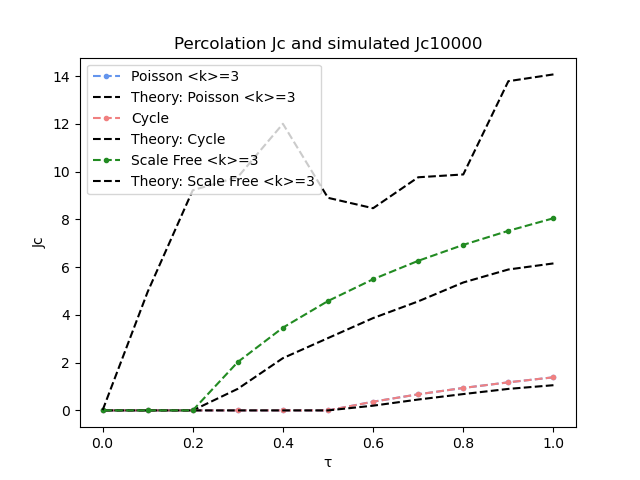
\includegraphics[width=\textwidth]{graficoJC}\caption{Confronto self percolation and simulation}
        \label{fig:graficoJC}
    \end{figure}

\subsection{Multiplex networks}\label{subsec:res-multiplex-networks}
    I risultati ottenuti dalla simulazione del modello multiplex sono mostrati in figura ~\ref{fig:diagram_phase}.
    Nei diagrammi di fase, notiamo che con un valore $\tau$ sufficientemente elevato, esiste sempre una soglia critica
    di $q$ oltre la quale è virtualmente impossibile arrestare l'epidemia.
    L'aumento di $t$ e $q$ comporta una diffusione dell'infezione sempre più ampia e difficile da contenere,
    poiché i valori di $Jc$ aumentano in modo significativo.
    Nella rappresentazione grafica del diagramma di fase,
    possiamo osservare come la curva della soglia di percolazione approssimi un'iperbole.

    \begin{figure}[H]
        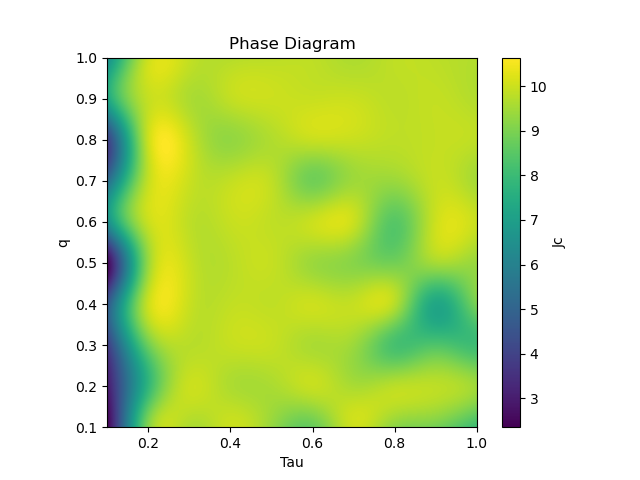
\includegraphics[width=\textwidth]{q_plot}\caption{Diagramma di fase al variare di q e $\tau$}
        \label{fig:diagram_phase}
    \end{figure}
